\documentclass[a4paper, dvipsnames]{beamer}
\usepackage[utf8]{inputenc}
\usepackage[T1]{fontenc}
\usepackage[french]{babel}
\usepackage{graphicx}

\title{Une démo de Beamer}
\usetheme{Antibes}
\usecolortheme[named=SeaGreen]{structure}
\setbeamercovered{transparent}

\begin{document}

\section{Introduction}

\begin{frame}
	\titlepage
\end{frame}    

\subsection{Mon premier transparent}
\begin{frame}{Mon premier transparent}
	\begin{columns}[c]
		\column{.5\textwidth}
		\only<1>{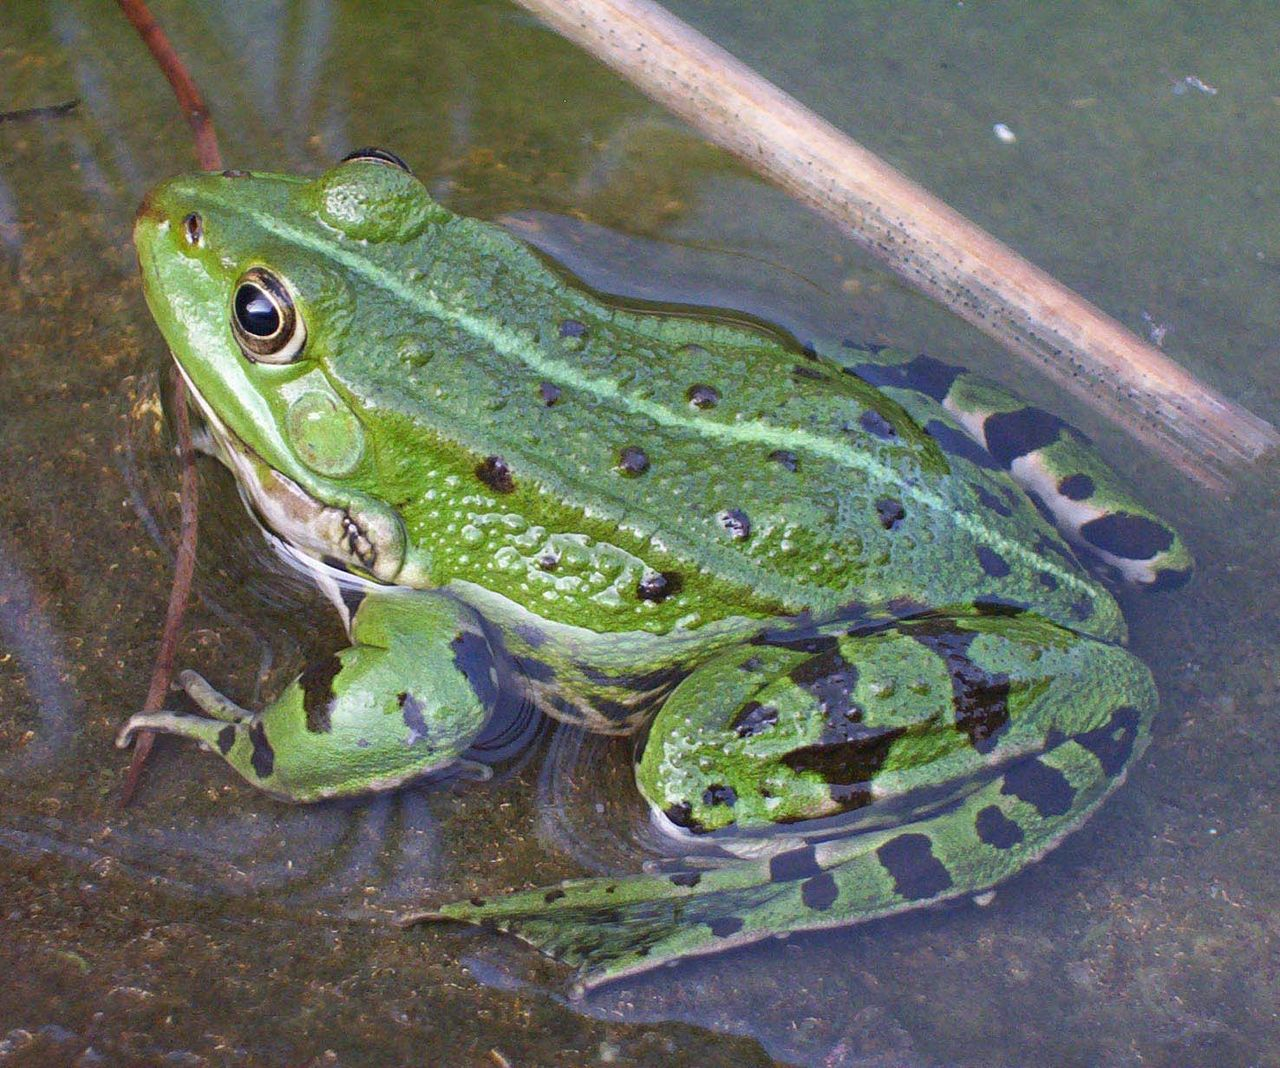
\includegraphics[width =\textwidth]{figures/frog.jpg}}
		\only<2>{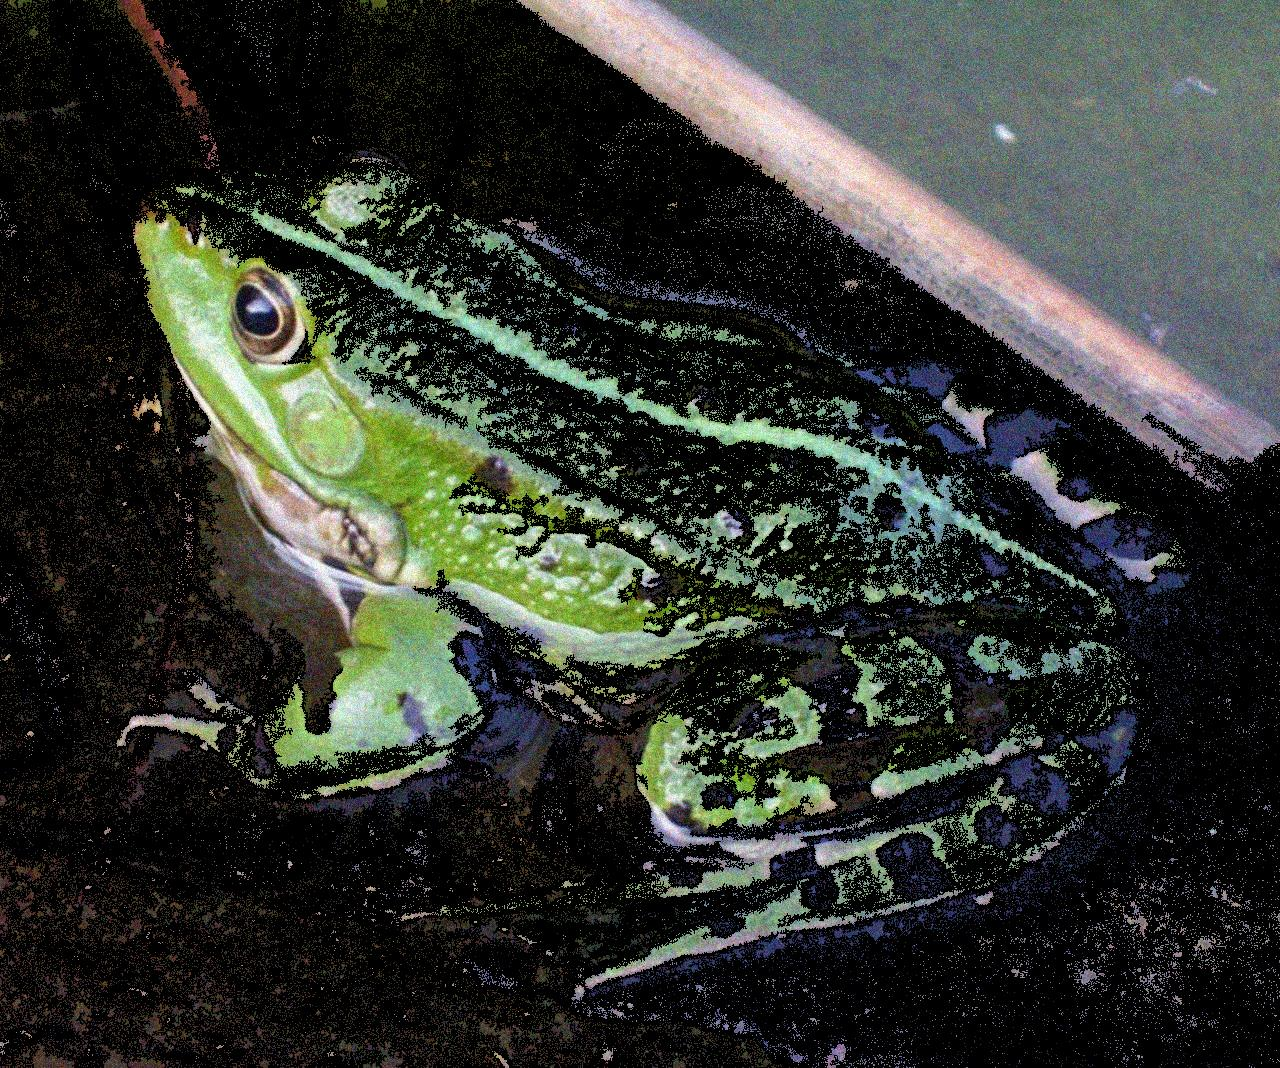
\includegraphics[width =\textwidth]{figures/frog_blur.jpg}}
		\column{.5\textwidth}
		\begin{block}{A savoir}
			\begin{itemize}
				\item Faire des slides (frames)
				\item Faire des blocks
				\item Faire des colonnes.
			\end{itemize}
		\end{block}
		\begin{alertblock}{A savoir}
			\begin{itemize}
				\item <1-> Des grenouilles
				\item <2->Modifiées !
			\end{itemize}
		\end{alertblock}
	\end{columns}
\end{frame} 


\end{document}